%%% mode: latex; mode:flyspell
%%%%%%%%%%%%%%%%%%%%%%%%%%%%%%%%%%%%%%%%%%%%%%%%%%%%%%%%%%%%%%%%%%%%%%%%%%%%% 
\section{Track momentum corrections}

The mean value of the reconstructed track momentum extrapolated to the tracker entrance is
slightly lower than the true MC momentum of the corresponding MC particle {\blue at the tracker entrance}.
The offset is \strike{of} {\blue on} the order of 30 keV/c and slightly \strike{different} 
{\blue depends on the ambiguity resolver used in the track fit.}
\strike{the track fits with different ambiguity resolvers.}
We correct the reconstructed \strike{momenta} {\blue momentum} of PAR tracks by 34 keV/c \strike{keV/c ,}
{\blue keV/c} and DAR tracks \strike{-} by 30 keV/c.

\begin{figure}[h]
\hspace{-0.6in}
\begin{tikzpicture}
  \node[anchor=south west,inner sep=0] at (0,0.) {
    % \node[shift={(0 cm,0.cm)},inner sep=0,rotate={90}] at (0,0) {}
    % \makebox[\textwidth][c] {
      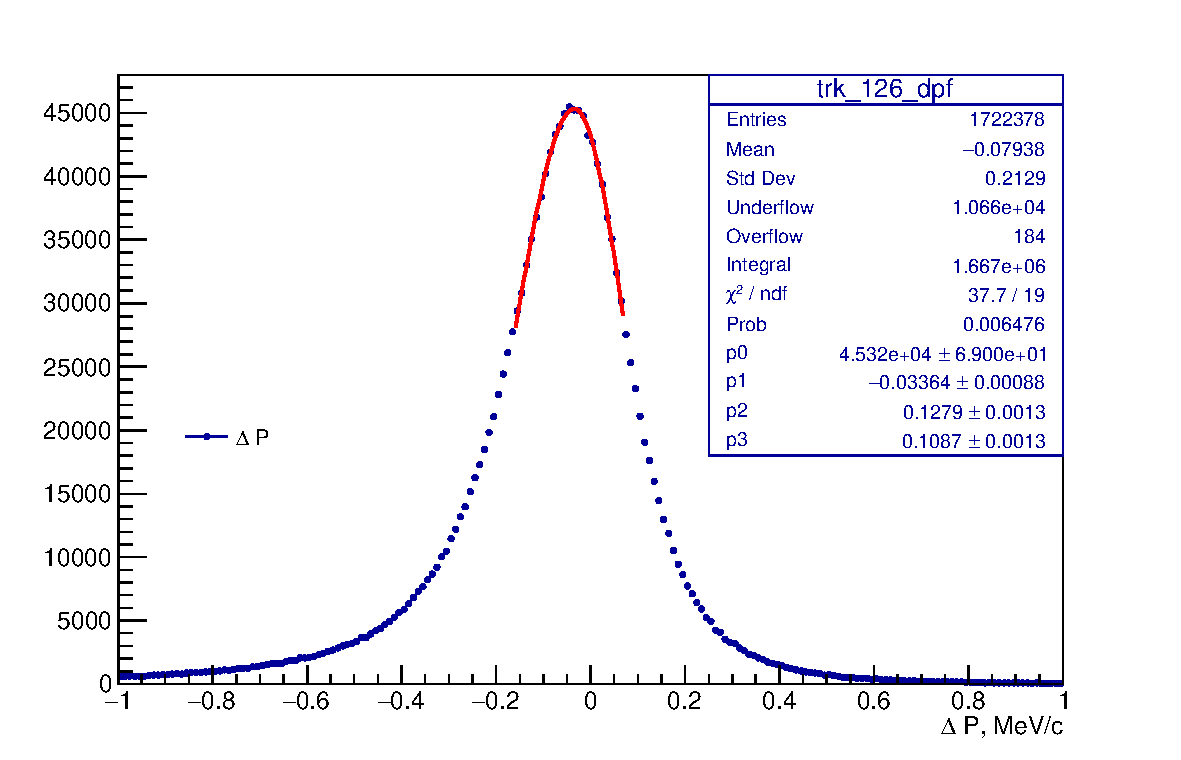
\includegraphics[width=0.6\textwidth]{figures/pdf/figure_00112_fele2s51b1_track_comp_ffff_1070_nocorr_trk_126_dpf}
    %}
  };
  \node[anchor=south west,inner sep=0] at (10,0.) {
    % \node[shift={(0 cm,0.cm)},inner sep=0,rotate={90}] at (0,0) {}
    % \makebox[\textwidth][c] {
      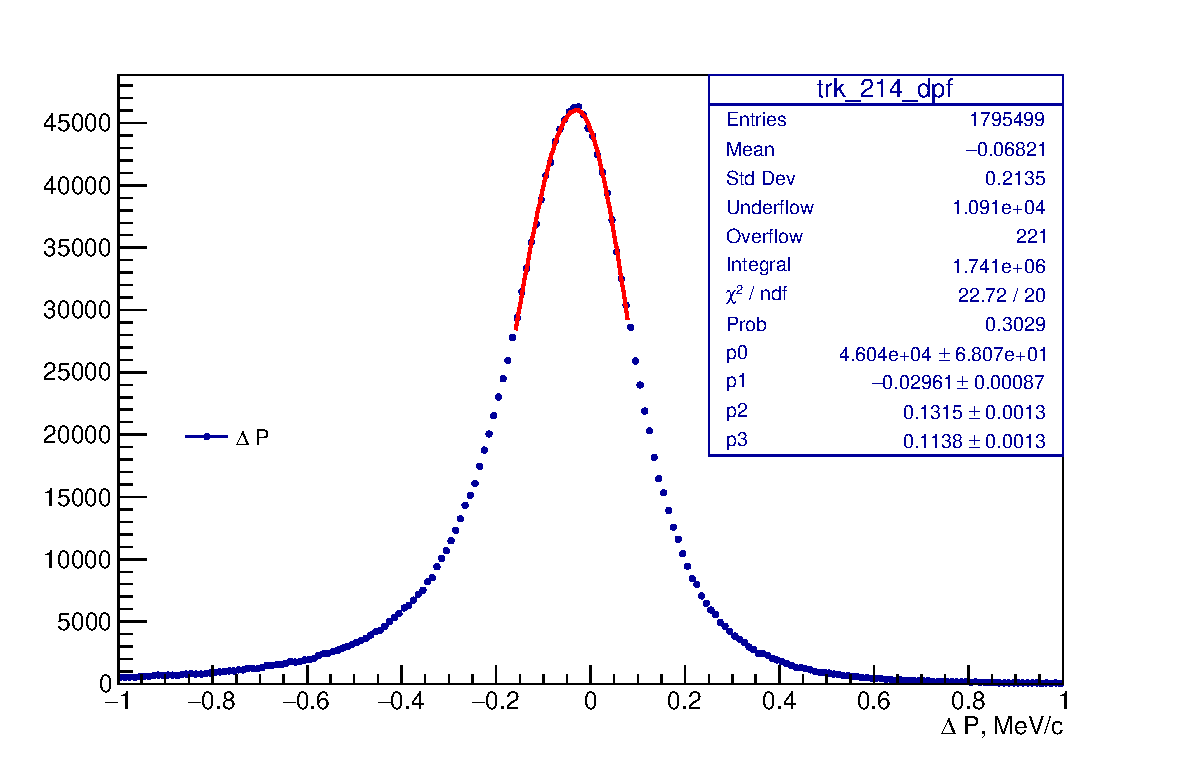
\includegraphics[width=0.6\textwidth]{figures/pdf/figure_00113_fele2s51b1_track_comp_ffff_1070_nocorr_trk_214_dpf}
    %}
  };
  % \node [text width=6cm, scale=0.8] at (4.5,6.4) {mu2e-18894 by Kevin Lynch and Jim Popp};
\end{tikzpicture}

\caption{
  \label{fig:sindrum_ii_fig_08_fit} 
  {\blue adjusted figure widths to reduce overlap}
  $\Delta P {\blue = P_{\rm rec} - P_{\rm MC}}$ distributions at the tracker front for PAR (left) and DAR (right) tracks. The distributions  
  are fit with \strike{the} {\blue an} asymmetric ($\sigma_{left} \ne \sigma_{right}$) \strike{g}{\blue G}aussian function. 
  {\blue The p}\strike{P}eak positions are used to correct the reconstructed \strike{momenta} {\blue momentum} of \strike{the} tracks 
  \strike{coming of} {\blue returned by} the respective fits.
}
\end{figure}


%%% Local Variables:
%%% TeX-master: "mu2e-36575"
%%% End:
